\documentclass[tikz, preview]{standalone}

\usepackage{tikz}
\usepackage[all,2cell]{xy}
\usetikzlibrary{matrix,arrows,shapes,decorations.markings}
\definecolor{rewritecolor}{rgb}{0,.9,1}
\tikzset{rewritenode/.style={shape=circle,fill=rewritecolor,scale=0.25,font=\Huge}}
\tikzset{RWopen/.style={shape=circle,draw=black,fill=white,scale=0.5,font=\Huge}}
\tikzset{RWclosed/.style={shape=circle,fill=black,scale=0.5,font=\Huge}}
\tikzset{CDnode/.style={shape=circle,fill=white,scale=.5}}
\tikzset{zxgreen/.style={shape=circle,draw,thick,fill=green}}
\tikzset{zxred/.style={shape=circle,draw,thick,fill=red}}
\tikzset{zxyellow/.style={shape=rectangle,draw,thick,fill=yellow}}
\tikzset{zxdiamond/.style={shape=diamond,fill=black,inner sep=2.75pt}}
\tikzset{->-/.style={decoration={markings,mark=at position .5 with {\arrow{>}}},postaction={decorate}}}


\begin{document}

\[
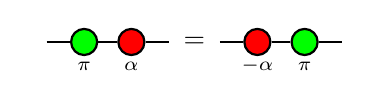
\begin{tikzpicture}
	%
	%
	%
	\node (v2) at (0,0) {$=$};
	%
	%
	%
	\begin{scope}[shift={(-0.1,0.3)}]
	\node [zxgreen,label={[shift={(0,-0.66)}]\scriptsize $\pi$}] (v1) at (-1.3,-0.3) {};
	\node (v3) at (-1.9,-0.3) {};
	\node [zxred,label={[shift={(0,-0.66)}]\scriptsize $\alpha$}] (v5) at (-0.7,-0.3) {};
	\node (v6) at (-0.1,-0.3) {};
	%
	\draw  (v5) edge [thick] (v6);
	\draw  (v5) edge [thick] (v1);
	\draw  (v3) edge [thick] (v1);
	\end{scope}
	%
	%
	%
	\begin{scope}[shift={(0.1,0.3)}]
	\node (v7) at (1.9,-0.3) {};
	\node (v10) at (0.1,-0.3) {};
	\node [zxred,label={[shift={(0,-0.7)}]\scriptsize $-\alpha$}] (v11) at (0.7,-0.3) {};
	\node [zxgreen,label={[shift={(0,-0.67)}]\scriptsize $\pi$}] (v12) at (1.3,-0.3) {};
	%
	\draw  (v10) edge [thick] (v11);
	\draw  (v11) edge [thick] (v12);
	\draw  (v12) edge [thick] (v7);
	\end{scope}
\end{tikzpicture}
\]



\end{document}
